\begin{frame}
    \frametitle{\problemtitle}
    \begin{block}{Problem}
      Given $n$ intervals $I_i=[\ell_i, r_i]$, for each of them find the length
      $v(I_i)$ of
      the longest \emph{chain} $I_i \subset I_{i_1} \subset I_{i_2}\subset \dots$.
    \end{block}
    \pause
    \begin{block}{Naive solution}
        \begin{itemize}
          \item<+-> $I_i \subset I_j$ is only possible if
             $r_i-\ell_i=t_i < t_j = r_j - \ell_j$.
          \item<+-> Sort by decreasing length and iterate over all longer
             intervals $\rightarrow$ $\mathcal O(n^2)$.
        \end{itemize}
    \end{block}
\end{frame}

\begin{frame}
    \frametitle{\problemtitle}
    \begin{block}{Problem}
      Given $n$ intervals $I_i=[\ell_i, r_i]$, for each of them find the length
      $v(I_i)$ of
      the longest \emph{chain} $I_i \subset I_{i_1} \subset I_{i_2}\subset \dots$.
    \end{block}
    \begin{block}{Solution}
        \begin{itemize}
          \item<+-> Sort by increasing $\ell$ first, and then decreasing $r$.
          \item<+-> The value $v(I_i)$ of $[\ell_i, r_i]$ is $1+\max_{\ell_j \leq \ell_i, r_i \leq r_j} v(r_j)$.
          \item<+-> Ignore $r_i$ if $r_i < r_j$ and $v(I_i) \leq v(I_j)$.
          \item<+-> What is left are increasing $r_i$ with decreasing $v$, that
             can be stored in an ordered set.
          \item<+-> Compute $v(I_i)$ by looking up the first element at least $r_i$.
          \item<+-> Insert $v(I_i)$ into the set and remove new suboptimal points
             that follow it.
        \end{itemize}
    \end{block}
\end{frame}

\begin{frame}
    \frametitle{\problemtitle}
    \begin{block}{Problem}
        Given $n$ intervals $I_i=[\ell_i, r_i]$, for each of them find the length
        $v(I_i)$ of
        the longest \emph{chain} $I_i \subset I_{i_1} \subset I_{i_2}\subset \dots$.
      \end{block}

    \vspace{1em}

    \begin{overprint}
      \onslide<1>
      \centering
      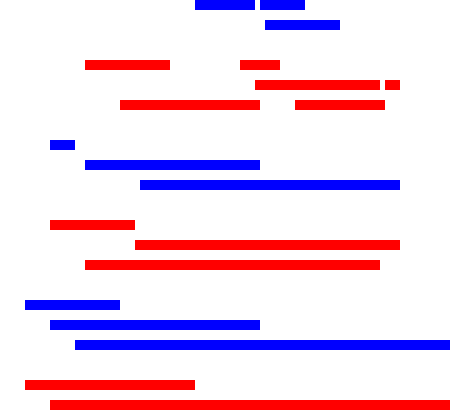
\includegraphics[height=0.6\textheight]{./visuals/1.png}
      \onslide<2>
      \centering
      
\includegraphics[width=0.8\textwidth]{./visuals/2.png}
      \onslide<3-4>
      \centering
      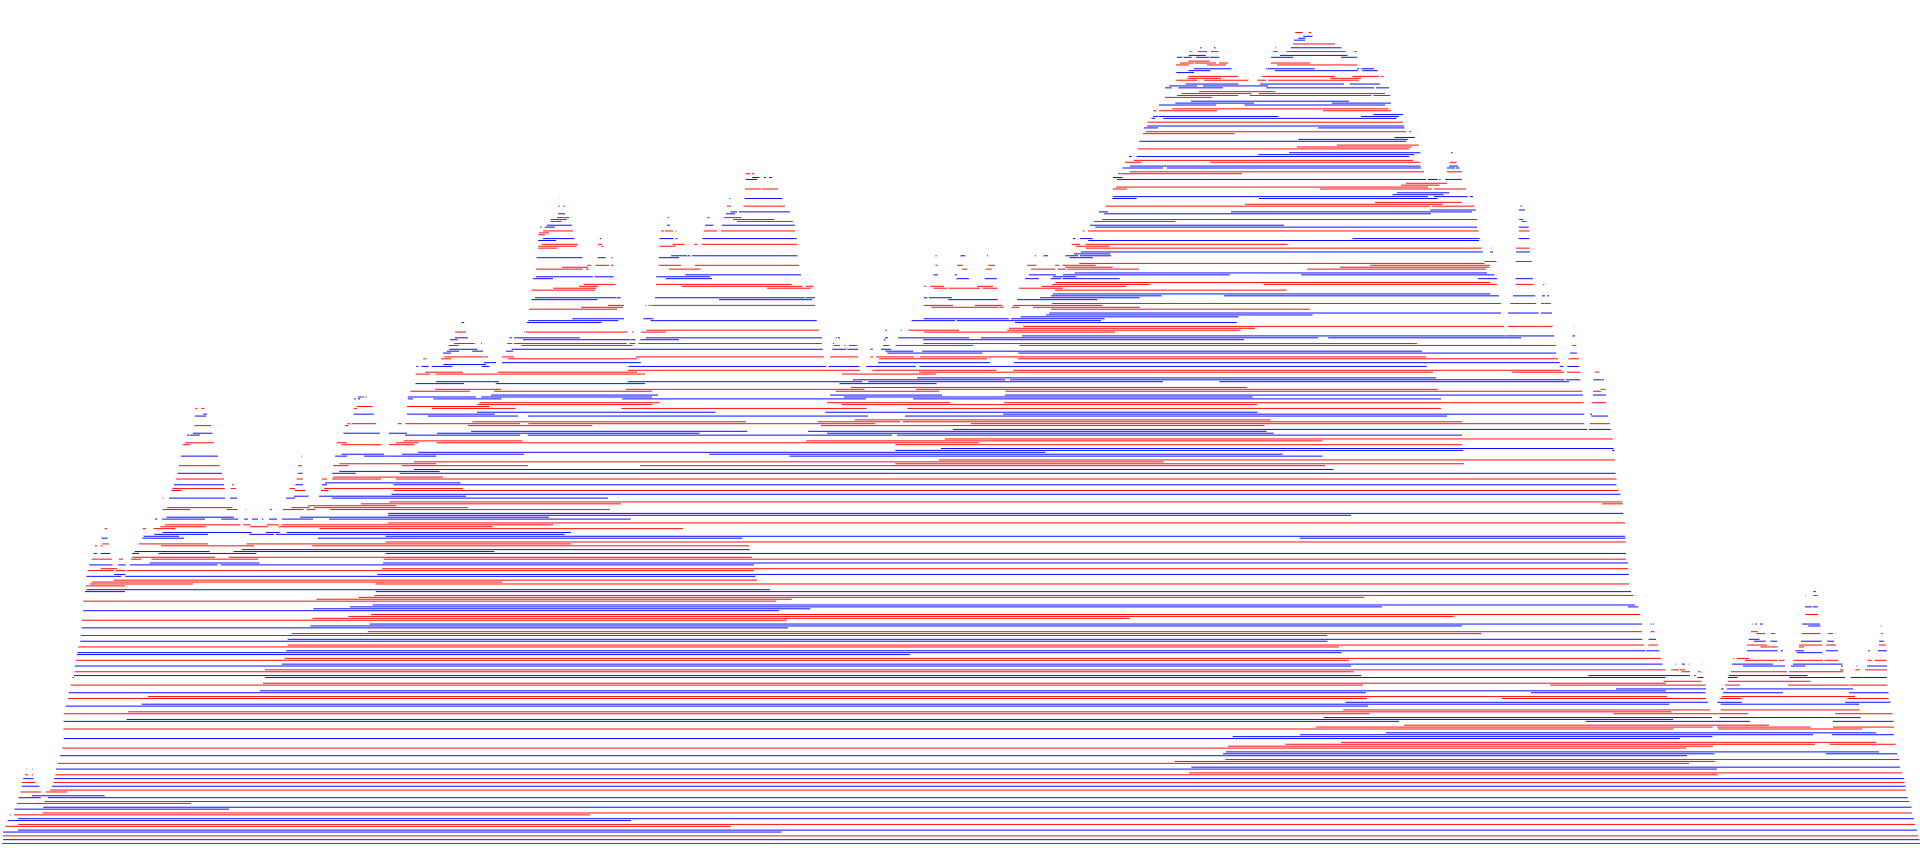
\includegraphics[width=0.8\textwidth]{./visuals/3.png}
    \end{overprint}
    \solvestats

\end{frame}
